\section{Auswertung}
Der erste Teil der Auswertung befasst sich mit der Fuorier-Synthese, der zweite mit der Analyse.
\label{sec:Auswertung}
\subsection{Fuorier-Synthese}
Wie schon in der Durchführung beschrieben, werden hier verschiedene Schwingungsmuster aus verschiedenen Oberwellen 
synthetisiert. Zuerst wird durch einstellen jeder ($1+2n$)-ten Oberwelle und Anpassung der Amplituden nach 
$\sfrac{1}{n}$ sowie der Phase versucht eine Rechtecksschwingung zu approximieren.
Dies funktioniert, so wie auch bei den anderen beiden, durch einzelnes Schalten der Phasenverschiebung um 90 oder 
180 Grad an den eingeschalteten Oberwellen.\\ \noindent
Für die Rechtecksschwingung wurden die als ungerade nummerierten Oberwellen eingeschaltet und das folgende Bild erzeugt.
\begin{figure}[H]
  \centering
  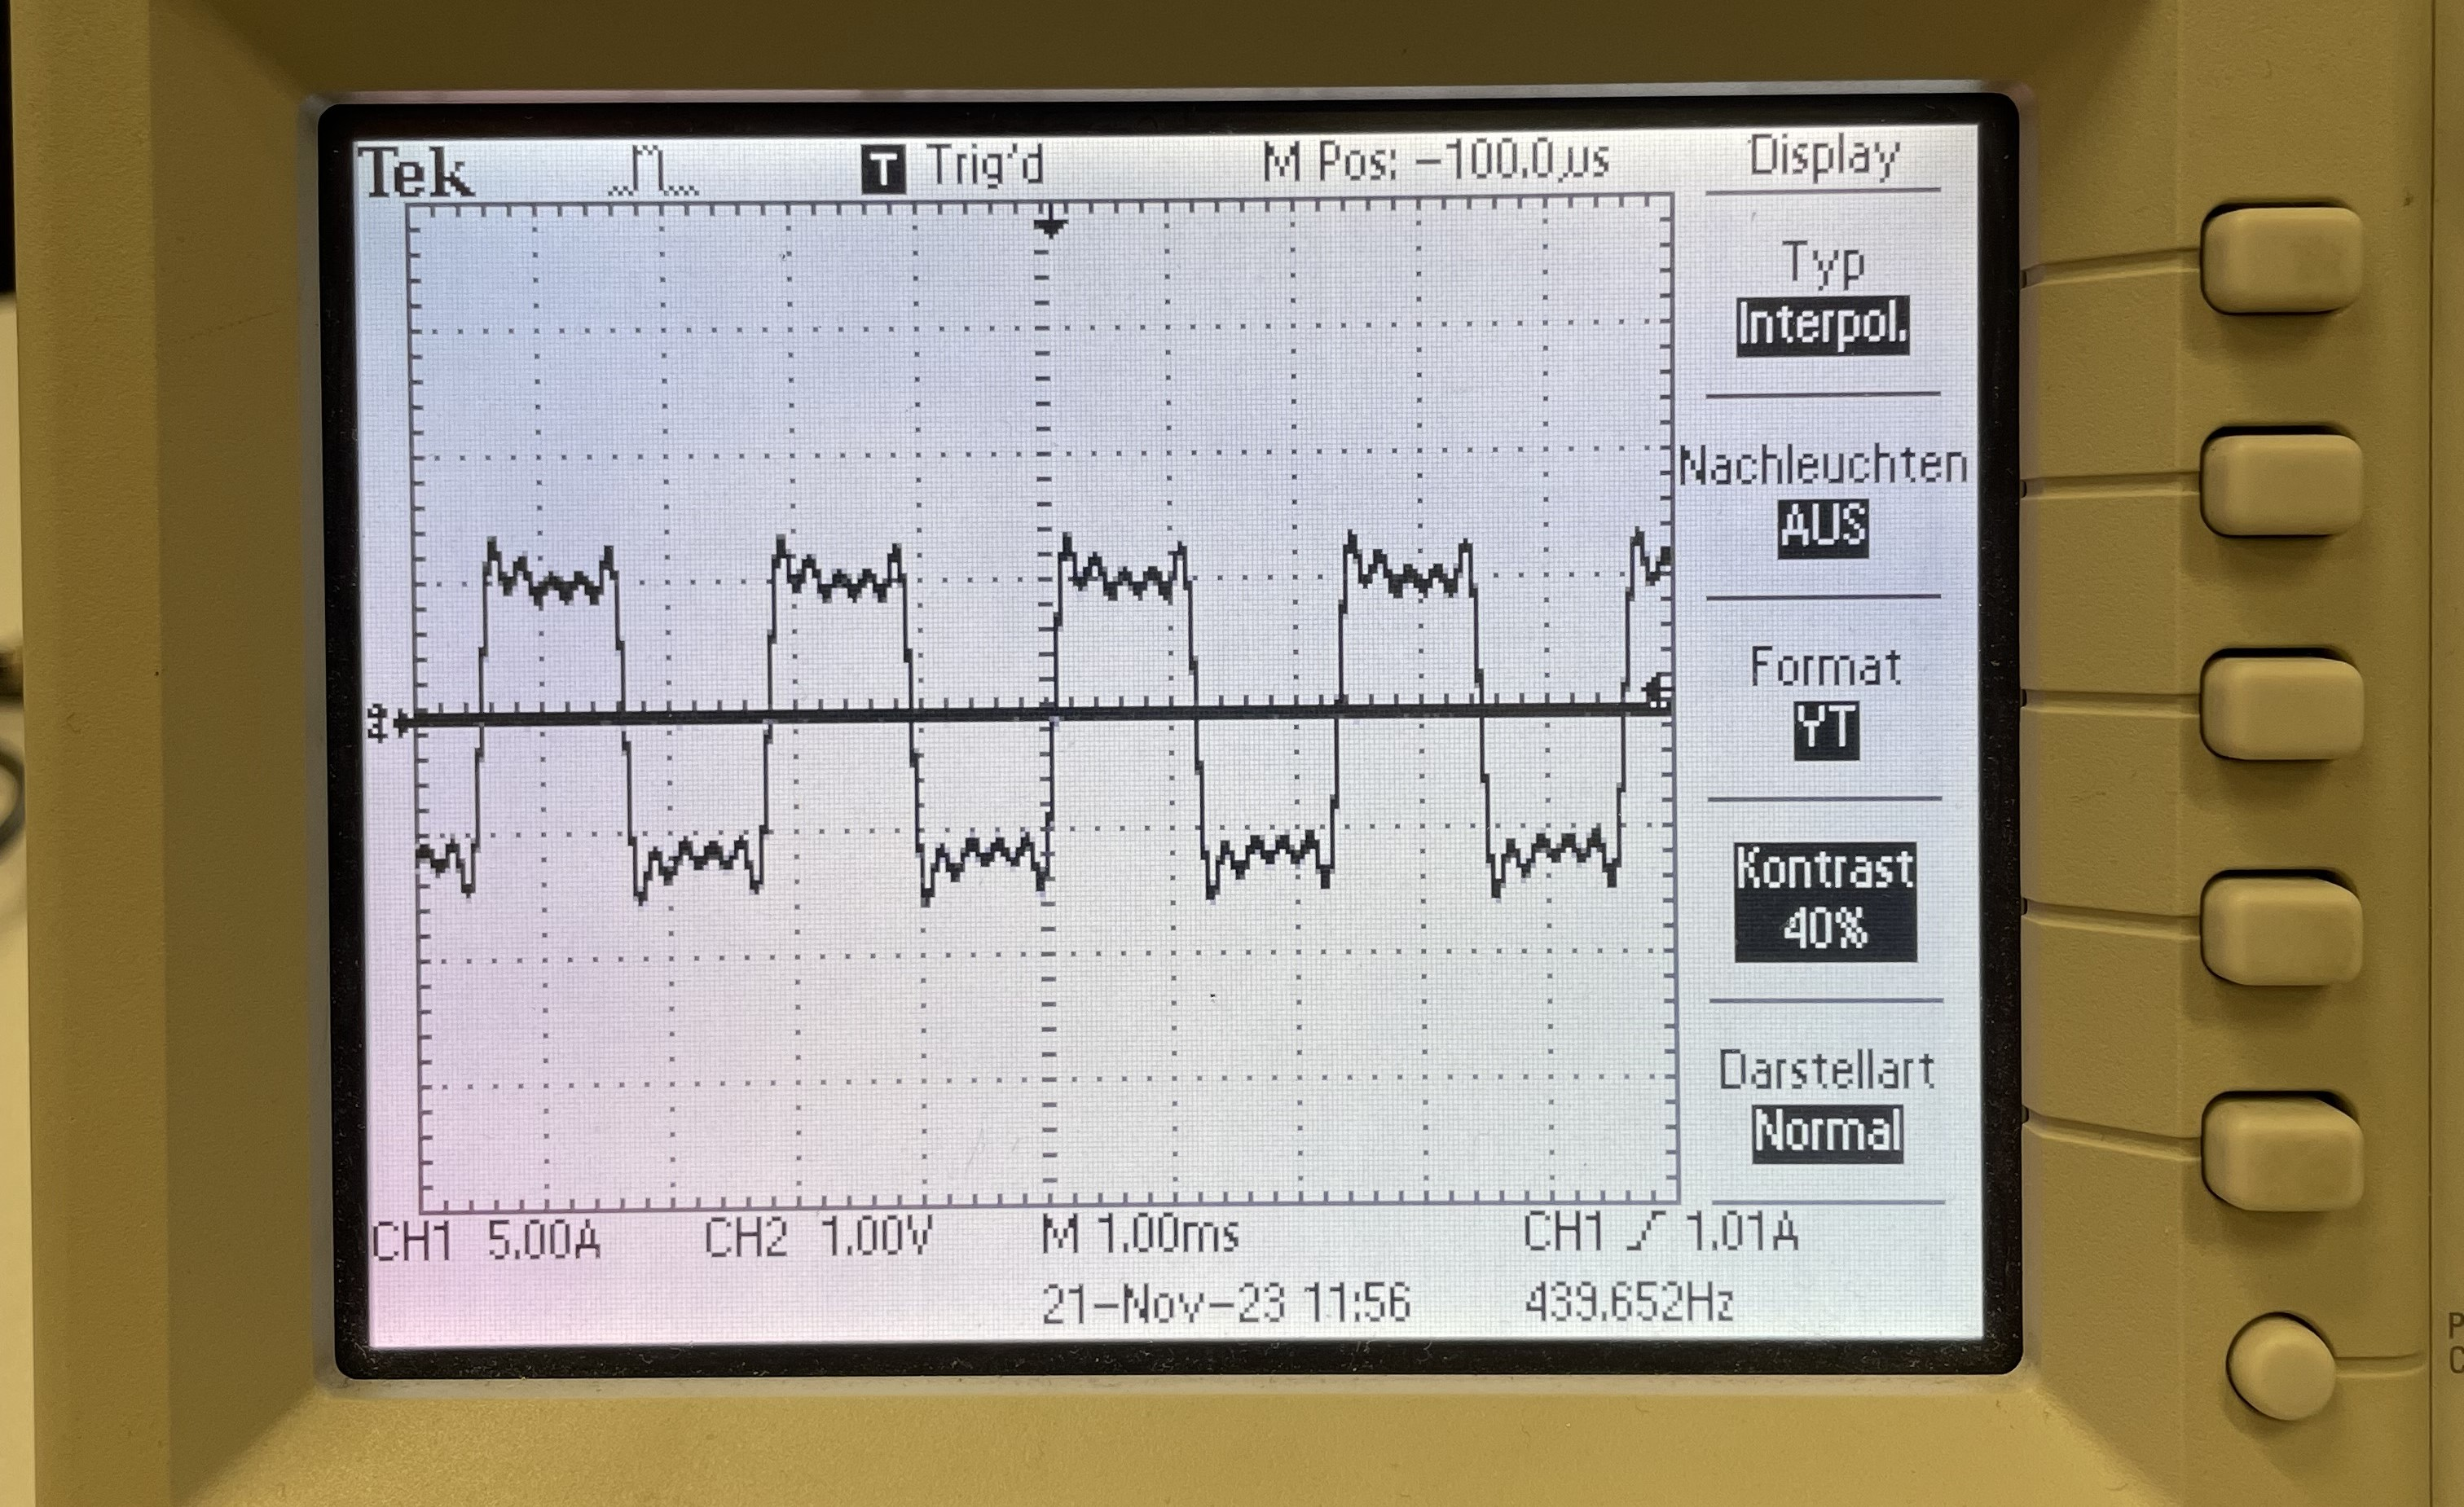
\includegraphics[scale=0.06]{Messdaten_Bilder/Rechtecksschwingung.jpeg}
  \caption{Synthetisierte Rechtecksschwingung.}
  \label{fig:Rechtecksschwingung}
\end{figure}\noindent
Da bei den letzten Oberwellen durch die kleine Amplitude ein hohes Rauschen im Bild des Oszilloskop durch die sehr kleine 
Amplitude zu verzeichnen war, wurden nicht alle möglichen Oberwellen zugeschaltet.
\begin{figure}[H]
  \centering
  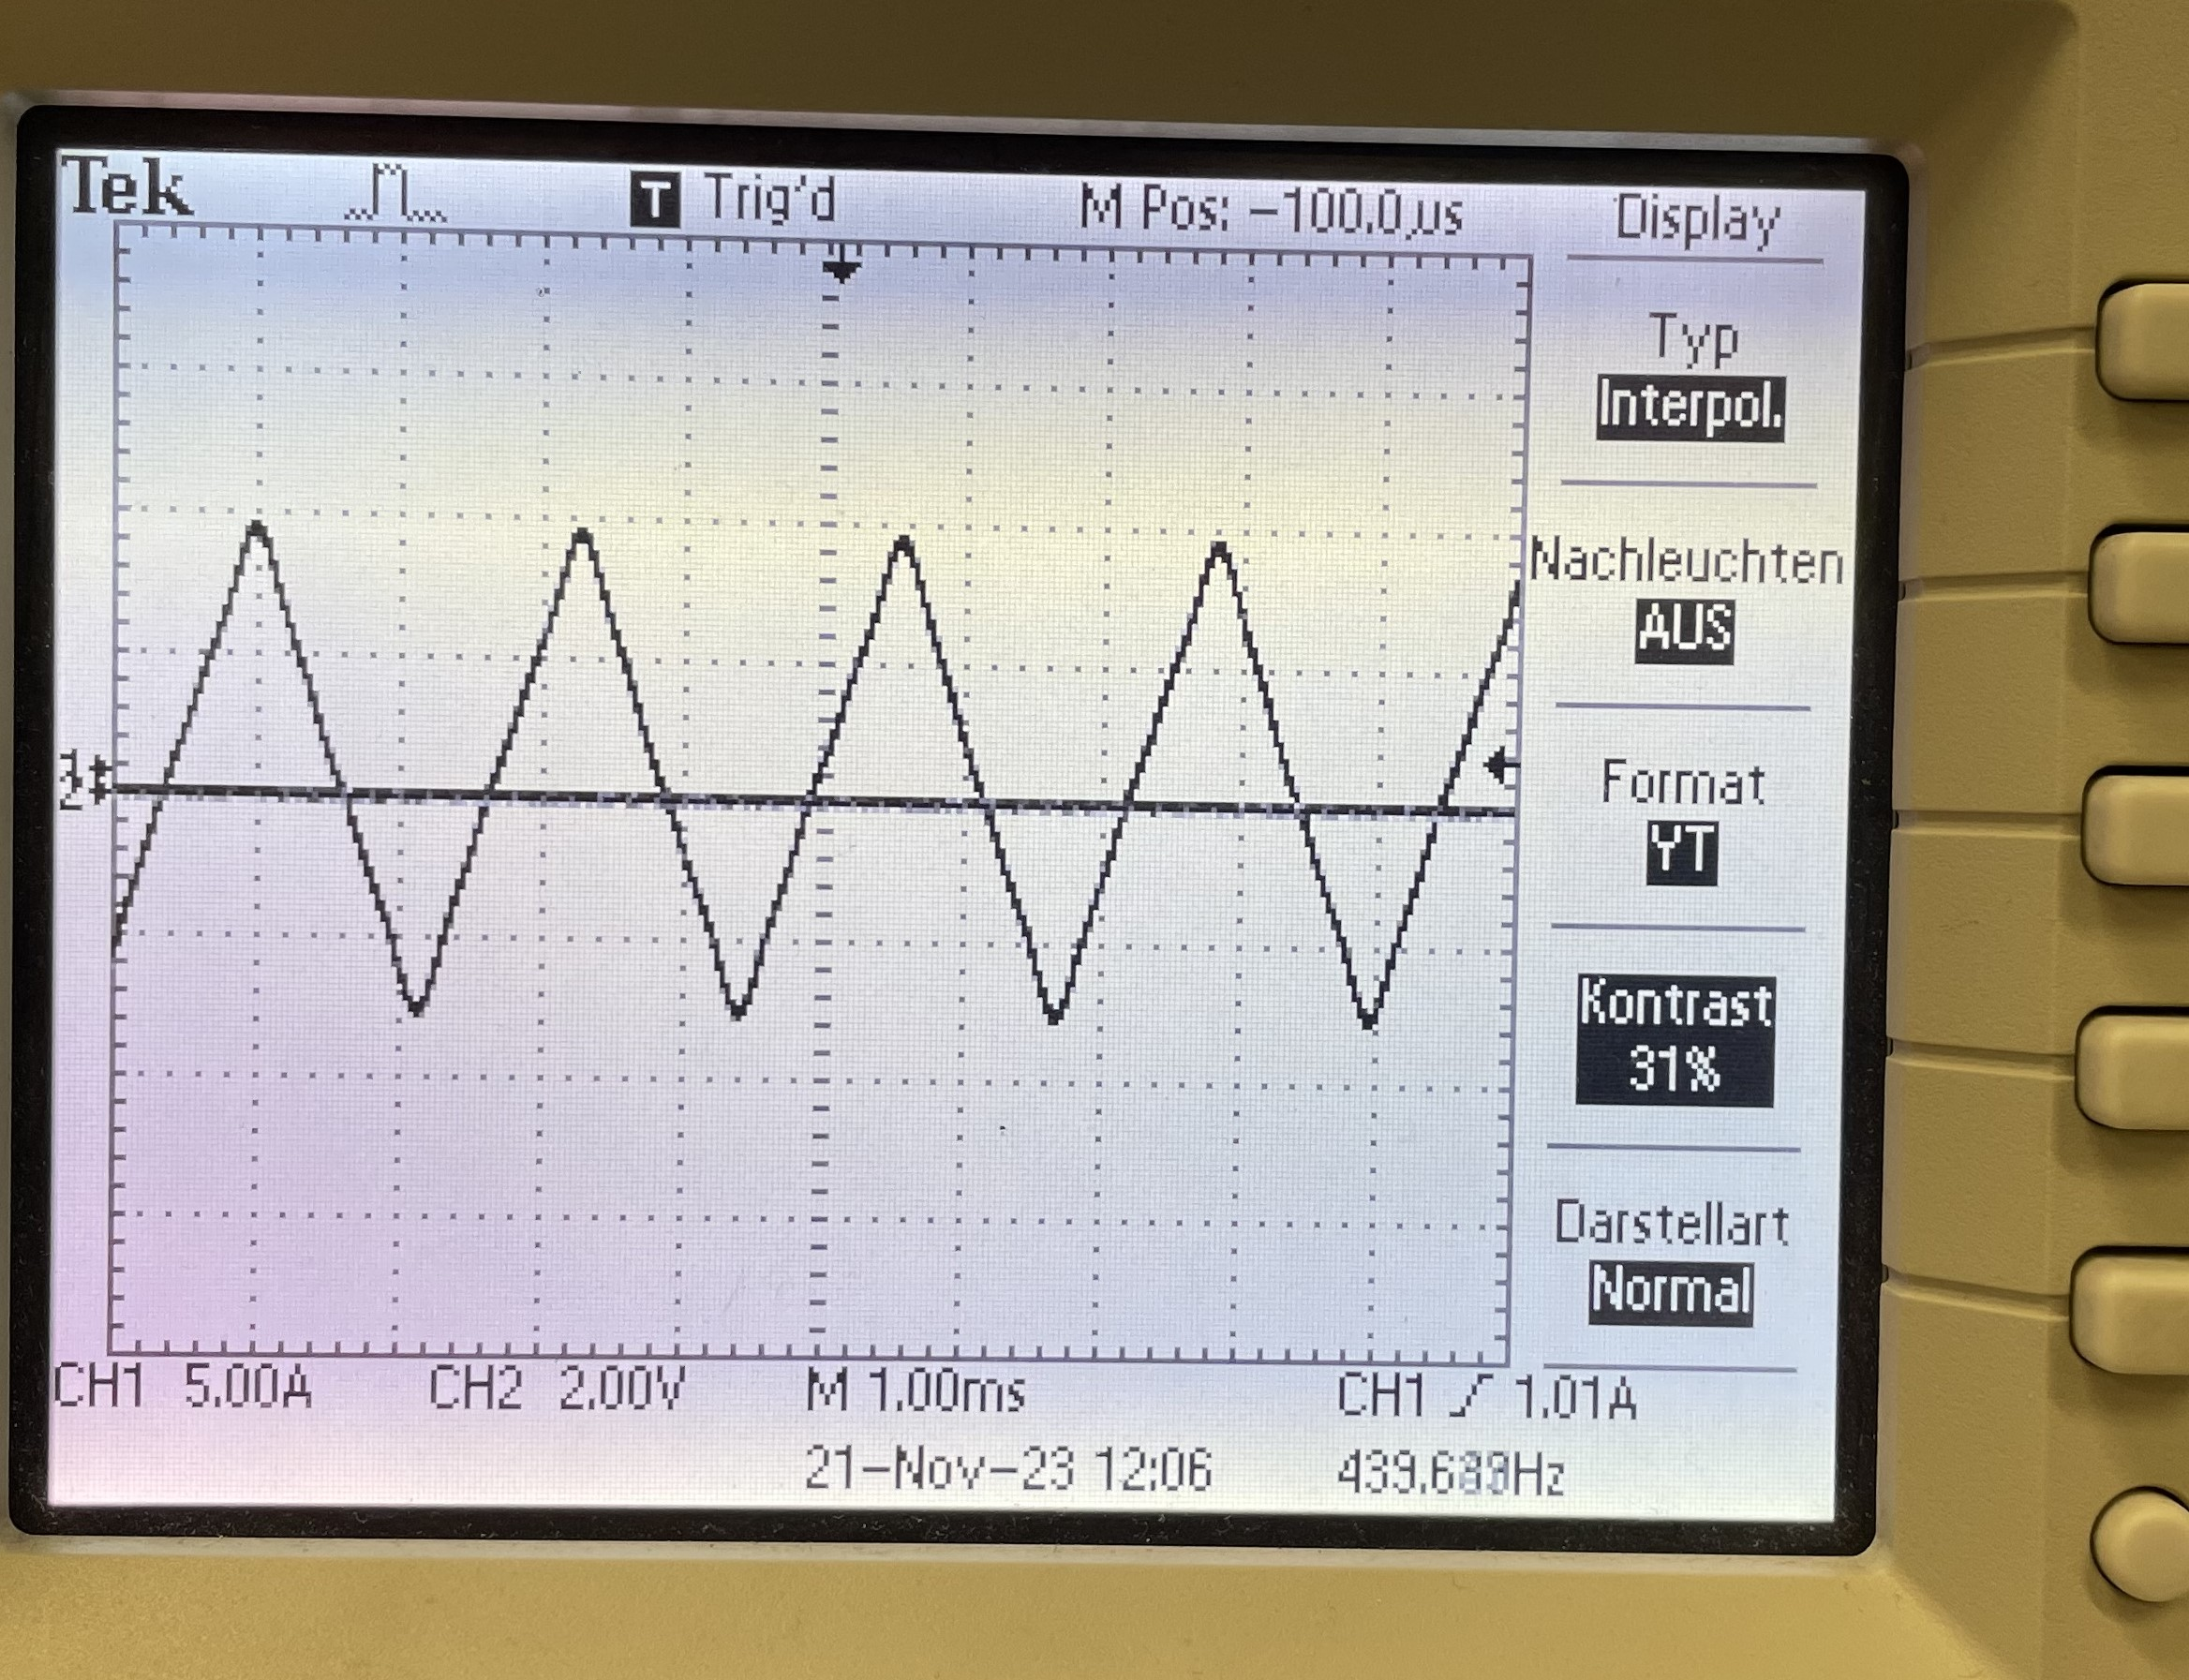
\includegraphics[scale=0.06]{Messdaten_Bilder/Dreiecksschwingung.jpeg}
  \caption{Synthetisierte Dreiecksschwingung.}
  \label{fig:Dreiecksschwingung}
\end{figure}\noindent
Die Dreiecksschwingung wird ebenfalls mit allen ungeraden Oberwellen generiert, jedoch fallen die Amplituden mit $\sfrac{1}{n^2}$.
Daher wird hier deutlich früher eine kleine Amplitude erreicht, weshalb auch deutlich früher ein starkes Rauschen auftritt. 
\begin{figure}[H]
  \centering
  \includegraphics[scale=0.06]{Messdaten_Bilder/Sägezahnschwingung.jpeg}
  \caption{Synthetisierte Sägezahnschwingung.}
  \label{fig:Sägezahnschwingung}
\end{figure}
\subsection{Fuorier-Analyse}
Da die Amplituden vom Oszilloskop in Dezibel angegeben sind, mussten diese zur Berechnung des Fits in Volt umgerechnet werden.
Dazu wird die Formel $1V=10{\text{dB}/20}$ genutzt. Diese ist zwar nur bis auf einen Vorfaktor korrekt, dieser ist jedoch zur Bestimmung
des Funkionsverlaufes vernachlässigbar.\\
Es sollen die $\sfrac{1}{n}$-Abhängigkeiten der verschiedenen Schwingungsmuster untersucht werden. Dazu werden die am Oszilloskop 
abgelesenen Messwerte geplottet und eine Funktion der Form $U(\nu)=a\cdot x^b$ gefittet. Der Koeffizent $b$ gibt Aufschluss über die 
besagte $\sfrac{1}{n}$-Abhängigkeit. Für die Fuorier-Analyse der Rechtecksschwingung wird ein Abfall von $\sfrac{1}{n^1}$ der Peaks
erwartet.
Mittels Python lässt sich folgender Fit plotten sowie die Koeffizienten $a$ und $b$ ermitteln.
Da die Amplituden vom Oszilloskop in Dezibel angegeben sind, mussten diese zur Berechnung in Volt umgerechnet werden.
Dazu wird die Formel $1V=10^{\si{dB}/20}$ genutzt. Dort fehlt zwar noch ein Vorfaktor, dieser ist jedoch zur Bestimmung
des Funkionsverlaufes vernachlässigbar. 
\begin{align*}
  a &= \si{896.8 ± 4.6}\\
  b &= (-1.003 ± 0.002)
\end{align*}
Es liegt also eine Kurve mit einer genäherten $\sfrac{1}{n}$-Abhängigkeit vor, so wie erwartet.
\begin{figure}[H]
  \centering
  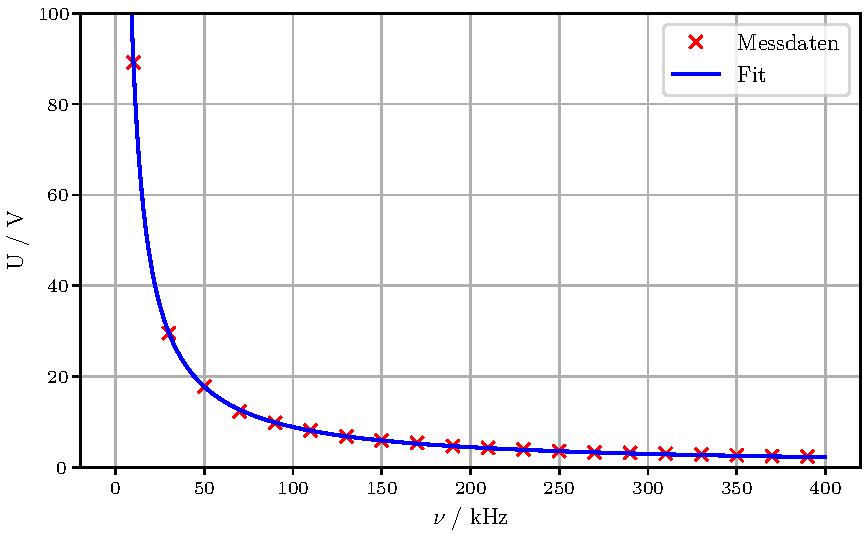
\includegraphics[scale=0.6]{plota.pdf}
  \caption{Plot 1.}
  \label{fig:Plot1}
\end{figure}\noindent
Wie schon diskutiert, fällt die Amplitude bei der Dreiecksschwingung mit $\sfrac{1}{n^2}$, sodass hier deutlich weniger Messwerte
abzulesen waren. Dieses Ergebnis spiegelt sich auch im Koeffizienten $b$ wieder.
\begin{align*}
  a &= \si{5570 ± 38.7}\\
  b &= (-1.996 ± 0.003)
\end{align*}
\begin{figure}[H]
  \centering
  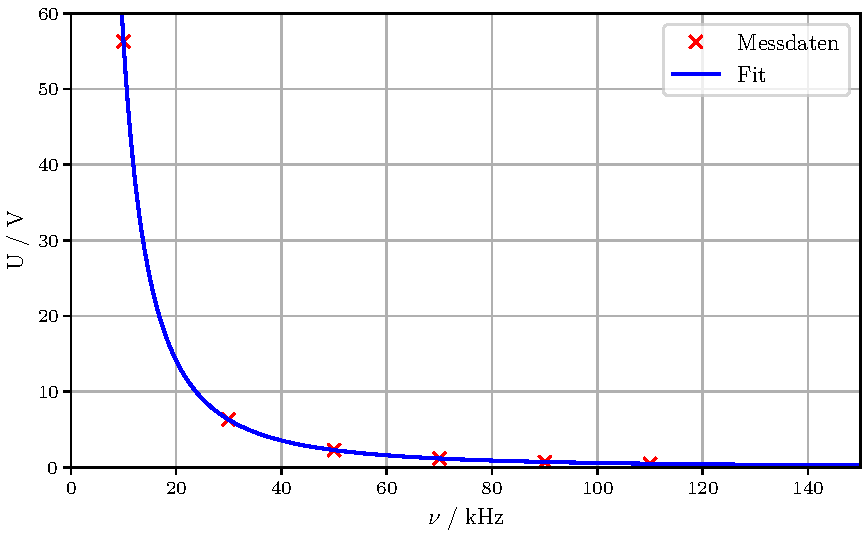
\includegraphics[scale=0.6]{plotb.pdf}
  \caption{Plot 2.}
  \label{fig:Plot2}
\end{figure}\noindent
Für die Sägezahnschwingung gibt es wieder deutlich mehr Messwerte, da wieder eine $\sfrac{1}{n}$-Abhängigkeit in der Kurve zu erwarten
ist und die Peaks im Abstand von 10\,kHz vorkommen.
\begin{align*}
  a &= \si{443.008 ± 2.415}\\
  b &= -0.997 ± 0.002
\end{align*} 
Wieder ist ein Koeffizient $b$ bestimmt worden, der sehr nah an dem Theorie-Wert liegt.
\begin{figure}[H]
  \centering
  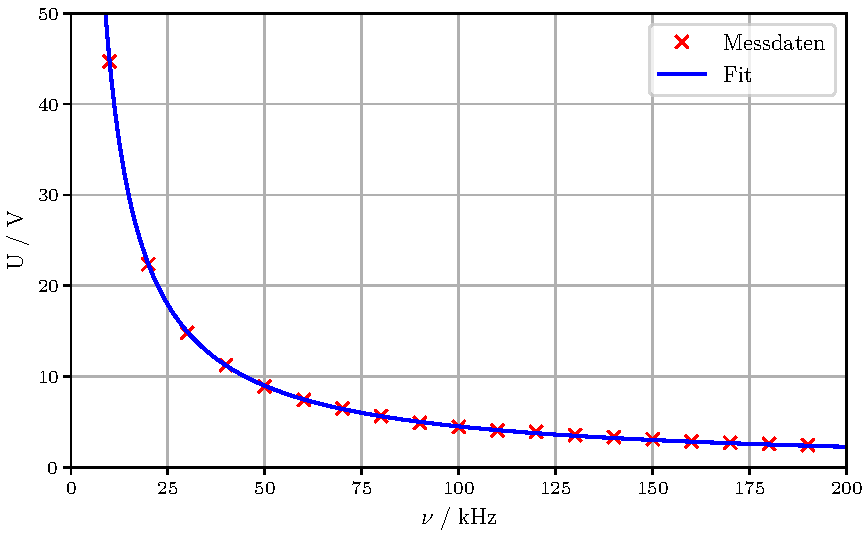
\includegraphics[scale=0.6]{plotc.pdf} 
  \caption{Plot 3.}
  \label{fig:Plot3}
\end{figure} 